

% intro to agent
Large language model agents \citep{wu2024autogen, hu2025owl, li2025search}, empowered by advanced LLMs \citep{guo2025deepseek, comanici2025gemini, yang2025qwen3}, have demonstrated competence in handling various real-world tasks. However, when faced with tasks requiring highly complex reasoning and multiple tools handling, even a minor error may ruin all the efforts \citep{press2023measuring}. To overcome the fragility of single-pass reasoning, recent research has increasingly integrated self-reflection mechanisms into agent architecture \citep{gou2023critic, shinn2023reflexion, zhou2023language}. Unlike standard CoT approaches, reflection enables agents to act as their own critics: scrutinizing past execution trajectories, diagnosing action-level errors, and iteratively refining their future strategies \citep{madaan2023self}.

\begin{figure}[t]
    \centering
    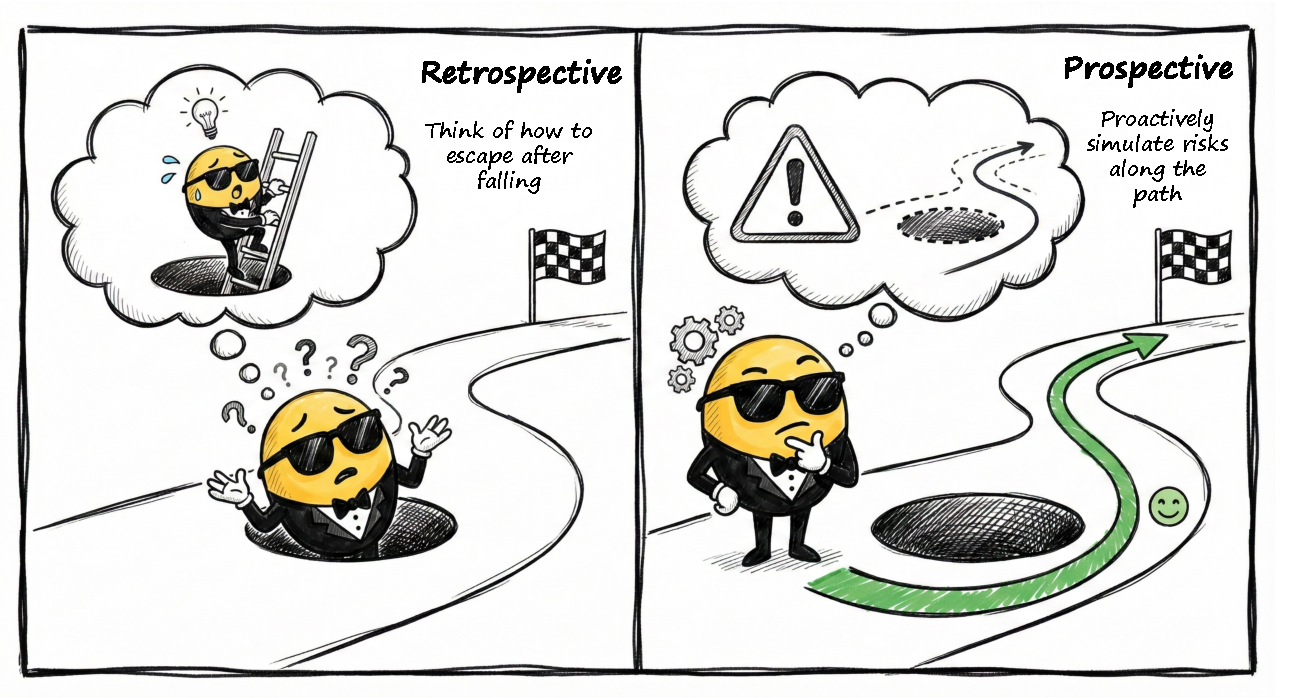
\includegraphics[width=0.95\linewidth]{img/pf_mot.pdf}
    \caption{\textbf{Retrospective vs. Prospective Reflection.} (Left) The retrospective agent triggers reflection only after encountering a failure. (Right) The prospective agent anticipates potential risks before execution, allowing it to adjust its plan and successfully bypass the obstacle.}
    \vspace{-15pt}
    \label{fig:mot}
\end{figure}

% weaknesses of existing reflection
Despite these advances, most existing reflection paradigms remain fundamentally \textbf{retrospective}, operating in a reactive manner that triggers correction only after failures have already occurred. While effective in some settings, such post-hoc reflection faces several inherent limitations in complex environments. Specifically, retrospective correction is often inadequate when actions produce \textbf{irreversible consequences}, such as accidentally deleting an important file. Additionally, diagnosing errors after execution can introduce substantial \textbf{trajectory-level noise}: by storing both failed attempts and subsequent fixes in memory, agents may suffer from contextual interference that destabilizes future decision-making. Furthermore, retrospective methods typically rely on repeated trial-and-error cycles, leading to significant computational cost and increased token latency as agents iteratively recover from mistakes.
% Therefore, these limitations underscore the necessity of a prospective capability to look ahead and anticipate potential pitfalls, ensuring a more effective and reliable agentic system.

To address these limitations, we propose \textbf{P}rospective \textbf{Reflect}ion (\textbf{\method}), a novel framework that shifts the reflection paradigm from reactive correction to proactive prevention, equipping agents with a prospective capability to anticipate potential pitfalls.
Central to this shift is identifying when reflection should intervene in the agent’s decision process. Existing methods typically reflect only after actions have been executed, when errors may already be costly or irreversible. In contrast, we observe that the planning stage provides a critical opportunity for proactive control: it is the point at which the agent commits to a strategy, yet has not begun to act on it.
Building on this insight, we introduce a planning-phase reflection mechanism that operates in the cognitive window between plan generation and action execution. By evaluating and revising plans before they are carried out, \method decouples error detection from irreversible outcomes, allowing agents to scrutinize their strategies for potential risks prior to execution.

  
However, the efficacy of prospective reflection is often constrained by the inherent difficulty of anticipating future failures. In the absence of structured guidance, aimless critique may even introduce more risks, such as hallucinations \citep{zhu2025llm}. To resolve this issue, we incorporate the ``Planning Errors'' into \method, which serves as an experiential anchor by distilling recurrent failure and success patterns from past agent trajectories. Specifically, upon generating a plan, the agent cross-references its proposed strategies against the planning errors to diagnose specific vulnerabilities such as hazardous tool usage. This guided reflection allows the agent to transform abstract foresight into concrete diagnosis by identifying semantic similarities between the current plan and historical pitfalls. Consequently, the agent can proactively substitute risky components with reliable alternatives, resulting in a robust and optimal trajectory that is empirically grounded before any action is committed to the environment.

Moreover, although the planning errors provide reliable and grounded references, proactively reflecting on future errors may still be insufficient under the uncertainty of complex environments. Relying solely on pre-execution critique can leave blind spots during execution and lead to oversights. Therefore, we incorporate a dynamic re-planning mechanism to complement planning-phase reflection by adaptively updating the agent’s plan during execution.  Unlike traditional architectures that adhere to rigid, fixed interval planning cycles, the dynamic re-planning continuously monitors the execution state to evaluate whether the current trajectory remains viable or necessitates a strategic shift. For instance, if the agent originally plans to search for a certain query while repeated failures, indicating infeasibility, the agent can trigger re-planning to revise its strategy and pivot toward alternative approaches.


Together, prospective reflection and dynamic re-planning form a unified framework that supports both proactive planning and robust execution.
To validate \method, we conduct comprehensive experiments across multiple benchmarks. Results show that \method achieves consistent performance improvements while maintaining reasonable token overhead. To sum up, our contributions are threefold:
 

 

 

\vspace{-15pt}
\begin{itemize}
\setlength{\itemsep}{-2pt}
    \item We propose \method, a prospective reflection framework that enables LLM agents to proactively identify and avoid critical failures before execution.
    % \vspace{-5pt}
    \item To further improve the effectiveness and efficiency of \method, we introduce two key components: the planning errors and  dynamic re-planning mechanism, which respectively provide experiential priors to assist reflection and adaptively revise plans during execution.
    % \vspace{-5pt}
    \item Extensive experiments demonstrate that \method significantly outperforms existing reflection-based baselines and competitive agent frameworks. Furthermore, transferability results show that \method generalizes across different agent architectures.
\end{itemize}
\vspace{-15pt}
